\section{Entwicklungsumgebung}
Es gibt zwei Entwicklungsumgebungen (IDE) von Xilinx, um den Zynq Ultrascale+ SoC zu programmieren und zu konfigurieren. Die eine ist Vivado. Vivado ist die IDE um Code für den FPGA zu entwickeln. Mit Vivado kann man IPs im Projekt einfügen, FPGA Code simulieren, synthetisieren, implementieren, den FPGA Konfigurieren und direkt auf dem FPGA debuggen.

Die zweite IDE ist Vitis. Mit Vitis kann man Code für das ARM-System schreiben, Bootdateien erstellen, das ARM-System programmieren, den FPGA konfigurieren und den ARM debuggen. Vitis basiert auf der Eclipse IDE mit den GNU GCC Tools.

In diesem Projekt wurden die Versionen 2019.2 von Vivado und Vitis verwendet. Es ist die erste Version von Vitis. Vorher wurde die Xilinx SDK verwendet um Code für den ARM zu schreiben. Ab Vivado 2019.2 ist es jedoch nicht mehr möglich Projekte für die SDK zu exportieren, da die SDK und Vitis unterschiedliche Files brauchen um die Hardware, welche mit Vivado generiert wird, zu importieren. Für beide Tools können mit TCL Skripte geschrieben werden.

Die Projekt von Vivado und Vitis beinhalten beide zum Teil absolute Pfade. Daher zeigte die Erfahrung, dass die Projekte nicht kopiert werden sollten, sondern mit Skripts gearbeitet werden soll. 

Mit den beiden Entwicklungsumgebungen kommt noch das Programm DocNav. Diesem Programm beinhaltet alle Dokumentationen von Xilinx.

\subsection{Vivado}
Vivado ist die IDE für die Entwicklung von FPGAs, sie versteht VHDL und Verilog. Vivado kann entweder im Projektmodus oder nicht im Projektmodus verwendet werden. In diesem Projekt verwenden wir Vivado nur im Projektmodus. Alle Befehle können entweder im GUI oder in der TCL Konsole eingegeben werden. Somit ist Vivado vollständig skriptbar. Ein Vivadoprojekt besitzt ein Top-Modul, welches alle anderen Module und Blockdiagramme hinzufügt.

Vivado besteht aus verschiedenen Teilprogrammen. Diese sind der IP-Integrator, der Simulator, der Synthetisierer, der Implementierer und der Hardwaremanager.

Die Dokumentation von Vivado ist auf verschiedene Dokumente aufgeteilt. Zum Starten ist die \textit{Vivado Design Suite User Guide: Using the Vivado IDE} gut geeignet. Diese Dokumentation referenziert in Kapitel zwei auf die weiteren Dokumentationen der einzelnen Unterprogramme von Vivado. \cite{vivado}

Der IP-Integrator ist das Tool um die Intellectual Properties (IP) zu instanziieren. Dafür erstellt der IP-Integrator ein Blockdiagramm, welches ein VHDL-Modul einbinden kann. Das Blockdiagramm kann auch selber erstellt IPs und VHDL-Module beinhalten, wobei hier die Grenze zwischen IP und VHDL-Modul schwimmend sind. Der Wizard "Create and Package new IP" kann die eigene Module in IPs umwandeln. Man kann jedoch VHDL-Module im Diagramm hinzufügen, ohne sie zu IPs generieren zu lassen. Zudem hat der Wizard Vorlagen für AXI-Schnittstellen. Diese sind in Kapitel \ref{sec:axi} genauer beschrieben. Der Wizard kann man in der Menuleiste unter Tools starten. Das IP \textit{zynq\_ultra\_ps} instanziiert das Prozessorsystem des Ultrascales. Somit kann man dieses konfigurieren und die anderen IPs an die Schnittstellen zum PS anhängen. Die Konfigurationen exportiert Vivado mit der XSA-Datei, mit welchem Vitis dann die Plattform generiert. \cite{vivado_ip}\cite{vivado_ip_integrator}

Für die Simulation können mehrere Sets definiert werden, welche man von einander getrennt aufrufen kann. Die Testbenches können direct auf die Module im Projekt zugreifen. \cite{vivado_sim}

Der Synthetisierer und Implementierer generieren das Bitfile für das Konfigurieren des FPGAs. Dabei ist der Synthetisierer der Hardware unabhängige Teil und der Implementierer der Hardware abhängige. Die XDC-Constraint-Dateien konfigurieren diese beiden Tools. In den Constraint-Dateien müssen auch die Zuweisung der Ein- und Ausgänge des Top-Moduls zu den Pins und deren Einstellungen stattfinden. \cite{vivado_const}\cite{vivado_synth}\cite{vivado_imp}

Der Hardware Manager kann den Bitstream direkt auf den FPGA laden und debuggen. Dafür braucht es jedoch noch einen oder mehrere Integrated Logic Analyser (ILA) IPs, welche im Blockdiagramm eingefügt werden können. Mit diesen kann man auf ein Trigger die gewünschten Signale für eine gewisse Zeit anschauen. \cite{vivado_debug}\cite{ila}

\subsection{Vitis}

\begin{figure}[tb]
    \centering
    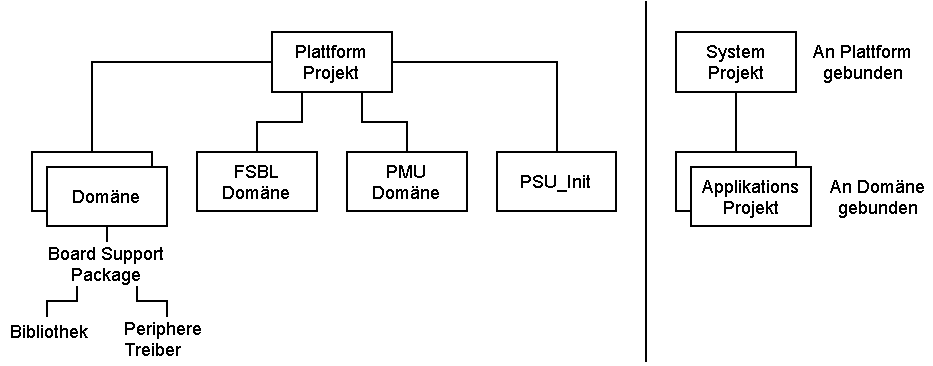
\includegraphics[width=\linewidth]{vitis}
    \caption{Zusammenhänge der verschiedenen Vitis-Projekten}
    \label{fig:vitis}
\end{figure}

Vitis ist die IDE von Xilinx, um das Prozessorsystem zu programmieren. Vitis basiert auf der Eclipse IDE. 
Von Vivado kann man die Hardware exportieren und in Vitis importieren. Mit der importierten Hardware wird ein Plattform-Projekt generiert. Diese Plattform beinhaltet Domänen und die Domänen wiederum Board Support Packages, welche die Bibliotheken und Peripherietreiber beinhalten. Jede Domäne ist für einen bestimmten Prozessorkern. Es können verschiedene Domänen für die selben Kerne existieren, wobei diese nicht die gleichen Einstellungen der Bibliotheken haben müssen. Zudem gibt es noch zwei spezielle Domänen. Eine Domäne für den First Stage Boot Loader (FSBL) und eine für die Firmware der Plattform Management Unit (PMU). Auf Grund von den Plattformen kann man Projekte erstellen. Hier gibt es auch zwei verschiedene Arten. Die Applikations-Projekte und die System-Projekte. Jedes System-Projekt kann mehrere Applikations-Projekte enthalten. Jedoch pro Prozessorkern nur eines. Jedes System-Projekt ist an ein Plattform-Projekt gebunden und jedes Applikations-Projekt an eine Domäne und befindet sich in einem System-Projekt.

Kompiliert wird der Code mit den GCC Compilern. Diese werden mit Vitis mitinstalliert und können von Vitis aus gestartet werden. Der Compiler generiert ELF-Dateien, welche auf den SoC geladen werden können. Die Erfahrung hat gezeigt, dass Vitis stabiler läuft, wenn zuerst das Plattform-Projekt compiliert wird und erst danach die System- und Applikations-Projekte. Falls jedoch die Plattform nicht verändert wurde und sie nicht veraltet ist, muss sie nicht notwendig compiliert werden.

Das Bootgen Tool generiert aus den ELF-Dateien und Bitfiles ein bootbares Image. Mit diesen kann man den SoC booten. Dafür muss es entweder auf die SD-Karte geschrieben werden, oder über JTAG auf den SOC geladen werden. Zusätzlich kann mit dem Tool Program Flash das Bootimage auf das externe Flash des SoCs laden. Dafür wird das File über JTAG and das Flash übertragen.

Mit dem Xilinx Software Command-Line Tool (XSCT) können auch Skripte für Vitis geschrieben werden. Die XSCT kann entweder in Vitis geöffnet werden, oder direkt in einem Terminal. Das XSCT basiert wie Vivadoskripts auf TCL.

Die Dokumentation von Vitis ist online zu finden. \cite{vitis}

\subsection{Schnittstelle zwischen Vivado und Vitis}
Vitis erstellt seine Plattform aufgrund der exportierten XSA-Datei von Vivado. Diese Datei beinhaltet die Konfiguration für das ARM-System, welches im Zynq-IP eingestellt wurde. Genauer gesagt ist die XSA-Datei ein ZIP-Archive. Die Konfiguration heisst psu\_init und existiert als C-Modul und als TCL Skript. Das C-Modul wird vom FSBL verwendet, um das ARM-System zu initialisieren und das TCL-Skripte verwendet Vitis um über JTAG das System ohne FSBL zu konfigurieren. 
Wenn eine Änderung im Vivadoprojekt stattfindet, müsste die Plattform aktualisiert werden. Jedoch zeigte die Erfahrung, dass die Plattform-Aktualisierfunktion von Vitis nicht zuverlässig funktioniert. Daher wird empfohlen ein neues Projekt mittels einem Skript zu erstellen und mit dem weiterarbeiten. Beim exportieren der Hardware in Vivado kann der Bitstream mit exportiert werden oder nicht. Auch hier wird empfohlen den Bitstream mit der Hardware zu exportieren und anschliessend in Vitis importieren, da sich in der Erfahrung ansonsten Komplikationen ergaben.
